\section{Dosímetro Floating Gate}
% TODO: diseño, cuentas, consideraciones
El dosímetro FG se basa en un MOSFET con gate aislado (floating gate).
Esto significa que el gate normalmente retiene su carga por mucho tiempo.
Esto tiene aplicaciones comerciales en memorias no volátiles:
una vez que se coloca cierta carga (representando información) en el gate,
tiene permanencia y puede medirse en base a las curvas IV del MOSFET.

Para realizar dosimetría con un FG,
explotamos la descarga del gate debido a la radiación.
Antes de irradiar,
se coloca carga en el gate mediante una corriente de túnel 
(\figref{fig:cargafg}).
\figp{cargafg}{figuras/fg/esquemainyeccion.pdf}
{ Inyección de carga en el FG a través de una corriente de túnel.
La tensión en el inyector produce un campo eléctrico en su óxido de gate,
que facilita una corriente de túnel Fowler-Nordheim.
La carga que pasa al FG prende el transistor lector.}
Esta carga altera la tensión de gate, prendiendo el transistor lector.

La radiación incidente produce pares electrón-hueco en el óxido de gate, 
descargando el gate (\figref{fig:irradiacionfg}).
\figp{irradiacionfg}{figuras/fg/irradiacion.pdf}
{ Descarga del FG debido a pares electrón-hueco creados por
radiación.
Los huecos son atraídos a la carga negativa del FG y
se recombinan con la misma, descargándolo.}
Esto va apagando el lector,
reduciendo su corriente de drain si se aplica tensión constante
(\figref{fig:fg_vd_cte})
\figp{fg_vd_cte}{figuras/fg/lector_vd_cte.pdf}
{Variación de la corriente de drain del lector con la tensión de gate,
para distintos valores de $V_{sd}$.}
o aumentando su tensión de drain si se aplica corriente constante
(\figref{fig:fg_id_cte})
\figp{fg_id_cte}{figuras/fg/lector_id_cte.pdf}
{Variación de la tensión de drain del lector con la tensión de gate,
para distintos valores de $I_d$.}
Calibramos estas cantidades contra la dosis recibida para construir un
dosímetro.
%
\subsection{Trabajos previos (emprolijar)}
\cite{cesari_floating_2014} carga FG=4V en 5s con -18V.

\cite{tarr_sensitive_2004} carga entre -20V y -40V en 10s. También monitorea
Id@Vsd=100mV. Calculó 5mV/rad, midió 3mV/rad.
%
\subsection{Acoplamiento capacitivo}
Ya que el FG está aislado,
su tensión es función de la carga que almacena 
y de la capacidad entre este y otros nodos del circuito.
Sumando la carga en cada capacidad se llega a la relación
\begin{align}
    Q_{FG} &= (C_R + C_W) V_{FG} + C_C (V_{FG}-V_C) + C_I (V_{FG}-V_I)
    \label{eq:ccoupling}
\end{align}
\subsection{Sensibilidad}
Un modelo simple para predecir la sensibilidad del dosímetro es plantear que
todos los aislantes que rodean al floating gate le aportan una carga
proporcional a la dosis y al volúmen del aislante.
A su vez, cada aislante forma parte de un capacitor que aporta a la capacidad
total del FG y reduce su corrimiento de tensión para una carga dada.

Esto determina la variación de la sensibilidad con la geometría que rodea al
FG,
\begin{align}
    S = \deriv{V}{E} \propto \frac{\sum_i A_it_i}{\sum_j A_j/t_j}
    \label{eq:sensibilidad_fg}
\end{align},
con $A_i$ y $t_i$ las áreas y espesores de los óxidos que rodean al FG.
Tanto los óxidos de campo como de gate consisten de SiO$_2$,
de modo que la permitividad sale como constante.
\subsection{Diseño}
El desempeño del dosímetro depende de cocientes
de capacidades entre FG y distintos nodos del circuito. 
Estos cocientes se reducen a relaciones entre las áreas del lector,
inyector y FG.
Debido a limitaciones del proceso de fabricación,
las áreas tienen un valor mínimo y varían de a pasos discretos.
Por otro lado, hay un área total máxima para el dosímetro.
Para elegir las dimensiones óptimas,
exploramos el espacio de soluciones mirando dos parámetros de calidad:
sensibilidad a la radiación, y eficiencia de inyección.

La ecuación~\ref{eq:sensibilidad_fg} dice que la sensibilidad se maximiza
asignando mayor área al óxido más grueso,
que es el óxido de campo entre FG y el well del lector.

Por otro lado,
la ecuación~\ref{eq:ccoupling} dice que la tensión de túnel $V_{FG}-V_I$
se maximiza, para un $V_I$ dado,
minimizando la relación $C_I/C_{FG}$.
Dado que hay un área mínima para el inyector,
es necesario aumentar las otras capacidades para reducir esa relación.

Exploramos el espacio de soluciones
graficando las curvas de nivel de ambos parámetros en función de dos variables
de diseño:
la relación área lector / área inyector,
y la relación área de well del lector / área inyector.
Esto se ve en las figuras~\ref{fig:sensibilidad_fg}
y~\ref{fig:eficiencia_inyeccion}.
\fig{sensibilidad_fg}{figuras/fg/sensibilidad.pdf}
{Sensibilidad del floating gate en función de la relación de áreas de 
inyector ($A_I$),
lector ($A_R$) 
y well del lector ($A_W$).}
\fig{eficiencia_inyeccion}{figuras/fg/inyeccion.pdf}
{Fracción de la tensión de inyección que cae en el óxido del inyector,
en función de la relación de áreas de 
inyector ($A_I$),
lector ($A_R$) 
y well del lector ($A_W$).}
% TODO: dimensiones finales
\begin{figure}[p]
    \centering
    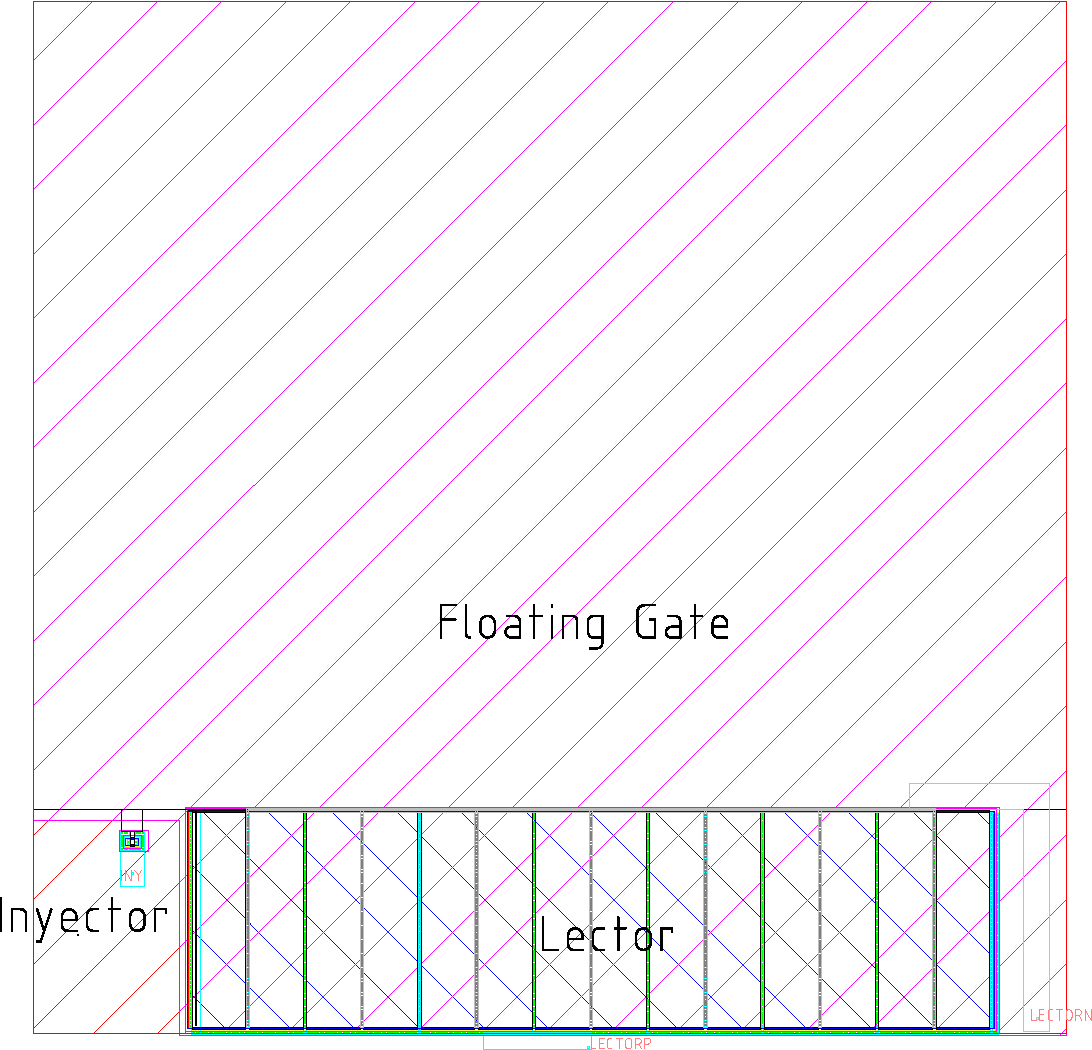
\includegraphics[width=\columnwidth]{figuras/fg/layout_hatch.pdf}
    \caption{Layout del dosímetro FG.}
    \label{fig:layoutfg}
\end{figure}
\subsection{Medición de la carga}
\fig{floatingcapacidades}{figuras/fgcapacidades/floatinggate2.pdf}{Modelo de
acoplamiento capacitivo en un MOSFET con floating gate.}
La tensión del floating gate controla el canal de un MOSFET.
Para determinar esa tensión usamos el acoplamiento capacitivo
\cita{pavan_floating_2004} 
entre floating gate y otros nodos, llegando a la ecuación
\begin{align*}
    V_{FG} &= \frac{C_I V_I + C_L V_L + Q}{C_I+C_L}
\end{align*}
con los términos ilustrados en la \figref{fig:floatingcapacidades}.

Durante la lectura se usa $V_I=V_R=0$.
En función de $V_{FG}$ y $V'_R$, la corriente del lector es
\begin{align*}
    I_R' &= \begin{cases}
        I_{D0} \left(\frac W L\right)_L
        \exp\left(\frac{V_{FG}-V_T}{nkT/q}\right)& V_{FG}>-V_T\\
        \beta_n\left(\frac W L\right)_L(V_{FG}+V_T+\frac{V'_R}2)V'_R &
        -V'_R-V_T<V_{FG}<-V_T\\
        \frac{\beta_n}2\left(\frac W L\right)_L(V_{FG}+V_T)^2 &
        -V'_R-V_T>V_{FG}.
    \end{cases}
\end{align*}
Estas ecuaciones nos indican que,
polarizando el lector con una tensión $V_{sd}$ pequeña
% FIXME: V_sd o V_r - V_{r'} ?
(usamos \SI{0.1}{\volt}),
estamos en la situación del medio y
la corriente de drain varía linealmente con $V_{FG}$
\subsection{Cargado del floating gate}
%
\subsubsection{Mecanismo de inyección}
Dado que el floating gate está aislado,
no intercambia carga en condiciones normales.
Por eso lo cargamos con una corriente de túnel
Fowler-Nordheim\cite{lenzlinger_fowlernordheim_1969}.
Aplicamos una tensión entre el gate y un transistor inyector.
Esto genera un campo eléctrico en el óxido de gate,
reduciendo el ancho de la barrera de potencial.
Así aumenta la probabilidad de túnel y en consecuencia la corriente
(\figref{fig:fowlernordheim}).
\fig{fowlernordheim}{figuras/fowlernordheim/fowlernordheim.pdf}
{Diagrama de bandas de la emisión de electrones del canal al gate de un MOS. 
El campo eléctrico en el óxido de gate reduce el ancho de la barrera de
potencial del óxido, facilitando el tuneleo.
Reproducido de \cite{lenzlinger_fowlernordheim_1969}}.

Esta corriente se ajusta a una expresión del tipo
\begin{align*}
    J_{FN} &= AF_{ox}^2\exp(-B/F_{ox}).
\end{align*}
El campo en el óxido $F_{ox}$ está dado por 
\begin{align*}
    V_{FG}-V_I &= F_{ox}t_{ox}+\psi_s+V_{FB},
\end{align*}
con $V_{FB}=(\Phi_S-\Phi_M)/e$ 
y $\psi_s$ la caída de tensión sobre el Si del inyector.

Para llevar el floating gate de 0V a una tensión negativa que prenda al lector,
aplicamos tensión negativa al inyector.
Si bien no controlamos $V_{FG}$ directamente,
reducimos su valor fijando $V_R=0$.
Así obtenemos una corriente electrónica de túnel hacia el floating gate.
Bajo esta polarización,
el inyector se encuentra en acumulación y se puede despreciar $\psi_s$.
%
%Nuestro proceso de fabricación alcanza breakdown del
%óxido de gate al aplicar \SI{13}{\volt}.
%A esta tensión la densidad de corriente es
%\SI{.1}{\nano\ampere\per\micro\meter\squared}, cargando nuestro floating
%gate a razón de \SI{3.9}{\volt\per\second}.
% TODO: calcular / medir curva Fowler-Nordheim
\subsubsection{Experimental}
\fig{medicion_fg}{esquematicos/medicion_fg/medicion_fg.pdf}
{Setup experimental para inyectar corriente en el FG,
con todos los caminos de pérdidas relevantes.
La conexión del sustrato a la guarda de la fuente de corriente
anula la tensión a través del diodo sustrato-bulk del inyector.}
Cargamos el floating gate aplicando corriente constante
entre el inyector y el well del lector.
Durante la inyección,
cualquier conductancia parásita entre esos nodos 
va a llevarse parte de la corriente,
reduciendo la carga inyectada.
Al mismo tiempo, parte de la carga proporcionada
va a cargar las capacidades del sistema.
Si aplicamos una corriente pequeña
(para cambiar lentamente la carga del FG),
el setup de inyección está la mayoría del tiempo cargando estas capacidades
hasta que se alcanza la tensión necesaria para el tuneleo de inyector a FG.

Usamos la guarda de la fuente de corriente para eliminar algunos caminos de pérdida
(\figref{fig:medicion_fg}).
Conectándola al sustrato evitamos la corriente en inversa del diodo de bulk
del inyector.
Ya que el inyector está bondeado al pin siguiente al well del lector,
no es posible interponer una guarda entre ellos para evitar pérdidas en el PCB.
\subsubsection{Curvas de carga y descarga}
La tensión del inyector (figuras~\ref{fig:descarga_inyector}
y~\ref{fig:carga_inyector})
varía linealmente mientras se carga la capacidad de los cables a corriente
constante.
Cuando alcanza una diferencia de potencial suficiente respecto del FG,
la corriente de túnel crece rápidamente y frena el crecimiento de la tensión.
Las curvas IV (figuras~\ref{fig:descarga_iv}
y~\ref{fig:carga_iv}) saturan a corrientes cada vez más grandes/chicas,
confirmando la variación de tensión del FG entre cada tramo
de inyección.
\fig{descarga_inyector}{figuras/fg/21a29dip_inyector.pdf}
{Descarga del FG midiendo tensión del inyector (línea punteada) y
corriente de drain del lector (línea sólida) a
$V_{sd}$=\SI{100}{\milli\volt}.
Esta corriente de drain es una indicación directa 
de la cantidad de carga en el FG.}
\fig{descarga_iv}{figuras/fg/21a29dip_iv.pdf}
{Curvas IV del lector medidas entre tramos de la descarga
    de la \figref{fig:descarga_inyector}.}
\fig{carga_inyector}{figuras/fg/12a21dip_inyector.pdf}
{Carga del FG midiendo tensión del inyector (línea punteada) y
corriente de drain (línea sólida) a
$V_{sd}$=\SI{100}{\milli\volt}.}
\fig{carga_iv}{figuras/fg/12a21dip_iv.pdf}
{Curvas IV del lector medidas entre tramos de la carga.}
\subsection{Irradiación con \Strontium}
Expusimos el dosímetro,
previamente cargado,
a una fuente de \Strontium.
La \figref{fig:irradiacionfg_respuesta} muestra que la corriente responde de
manera casi lineal a la dosis.
La variación de la sensibilidad se ve con más detalle en la
\figref{fig:irradiacionfg_sensibilidad}.
\fig{irradiacionfg_respuesta}{figuras/fg/irradiacion_corriente.pdf}
{Corriente del lector del FG polarizado con
    $V_{sd}$=\SI{100}{\milli\volt} en función de la dosis recibida.
    % TODO: mover al texto?
    % TODO: originalmente decia ``sensibilidad inicial'', cual es la correcta?
La corriente calculada parte de la corriente inicial extraída de la
medición.}
\fig{irradiacionfg_sensibilidad}{figuras/fg/irradiacion_sensibilidad.pdf}
{Sensibilidad del FG polarizado con
    $V_{sd}$=\SI{100}{\milli\volt} en función de la dosis recibida.
}
% TODO: tomar valor absoluto para aclarar que la sensibilidad aumenta
La sensibilidad cambia con la dosis debido a dos fenómenos opuestos.
\begin{itemize}
    \item A medida que se descarga el floating gate, disminuye el 
        campo eléctrico en el óxido y baja el yield de generación de pares 
        electrón-hueco.
    \item Al reducirse la corriente, crece $\frac{dI_D}{dV_G}$ 
        (\figref{fig:didv}) y esto aumenta la sensibilidad.
\end{itemize}
Se ve en las mediciones un crecimiento de la sensibilidad que se aplana al
alzanzar \SI{50}{\Gray}.
\fig{didv}{figuras/fg/didv.pdf}
{La pendiente de la curva $I_D(V_G)$ del lector aumenta a medida que $I_D$ cae,
incrementando la sensibilidad del FG.
Esta curva fue simulada con modelos provistos por el foundry,
debido a que la compuerta del dispositivo fabricado es inaccesible para
mediciones.}
\subsection{Corriente de ruido}
Establecimos que una medición con este dosímetro consiste en promediar 10
muestras de corriente.
Así podemos definir el ruido como la desviación estándar de este promedio.
Medimos la corriente del lector en ausencia de radiación y
tomamos la diferencia entre muestras sucesivas para eliminar derivas
(\figref{fig:ruidofg}).
Esto resulta en una desviación estándar
$\sigma=$ \SI{27}{\nano\ampere},
correspondiente a una dosis de \SI{4}{\milli\gray}.
\fig{ruidofg}{figuras/fg/ruido.pdf}{Diferencia entre
mediciones sucesivas de corriente del lector, escaladas para representar el
ruido en promedios de 10 muestras.}
% TODO: otra estimación de ruido/resolución
